\subsection{Line picking on the rectangle with the max metric}
\label{sec:rect_manhattan}

Example showing how a different distance metric can simplify the result: 

\begin{figure}[tbp]
  \begin{center}
    \subfloat[\label{fig:rect_max_pdf.]{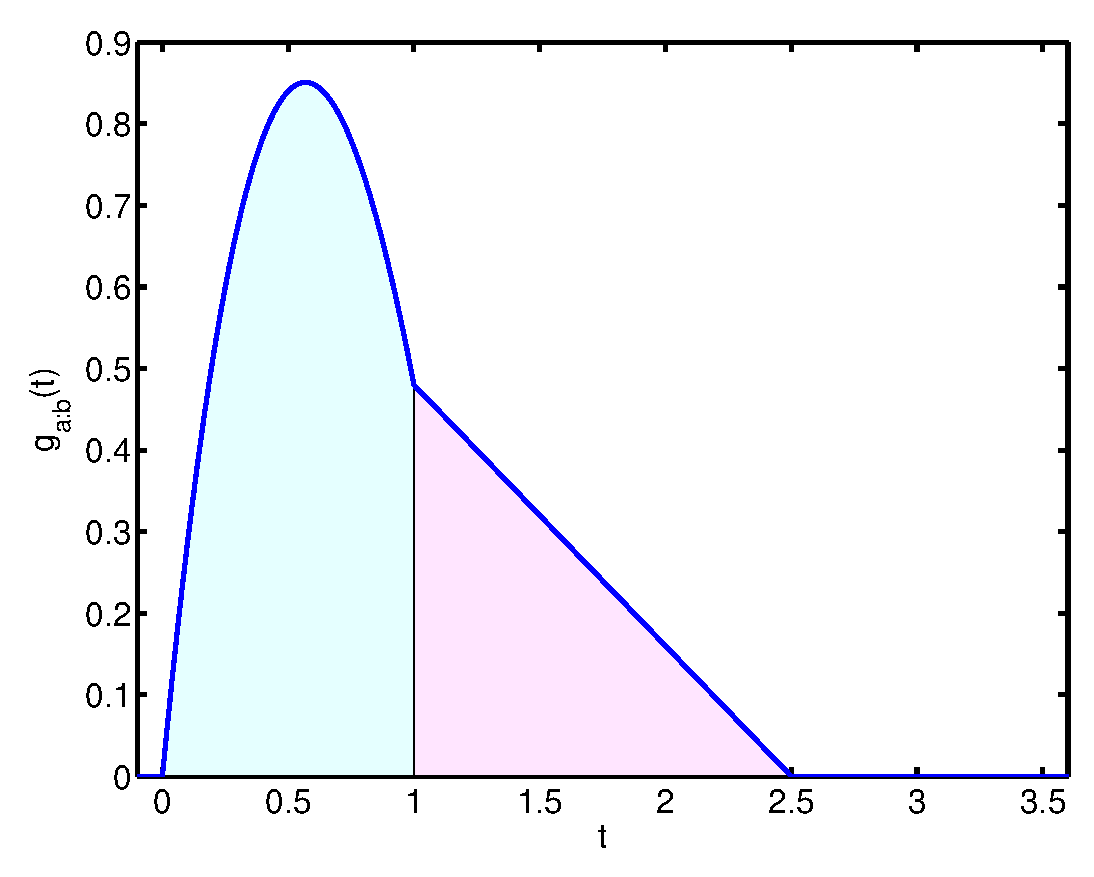
\includegraphics[width=0.48\columnwidth]{../Matlab/Plots/LinePicking_test_rect_max_regions.eps}}
      \hspace{3mm}
    \subfloat[\label{fig:rect_max_pdf_var.]{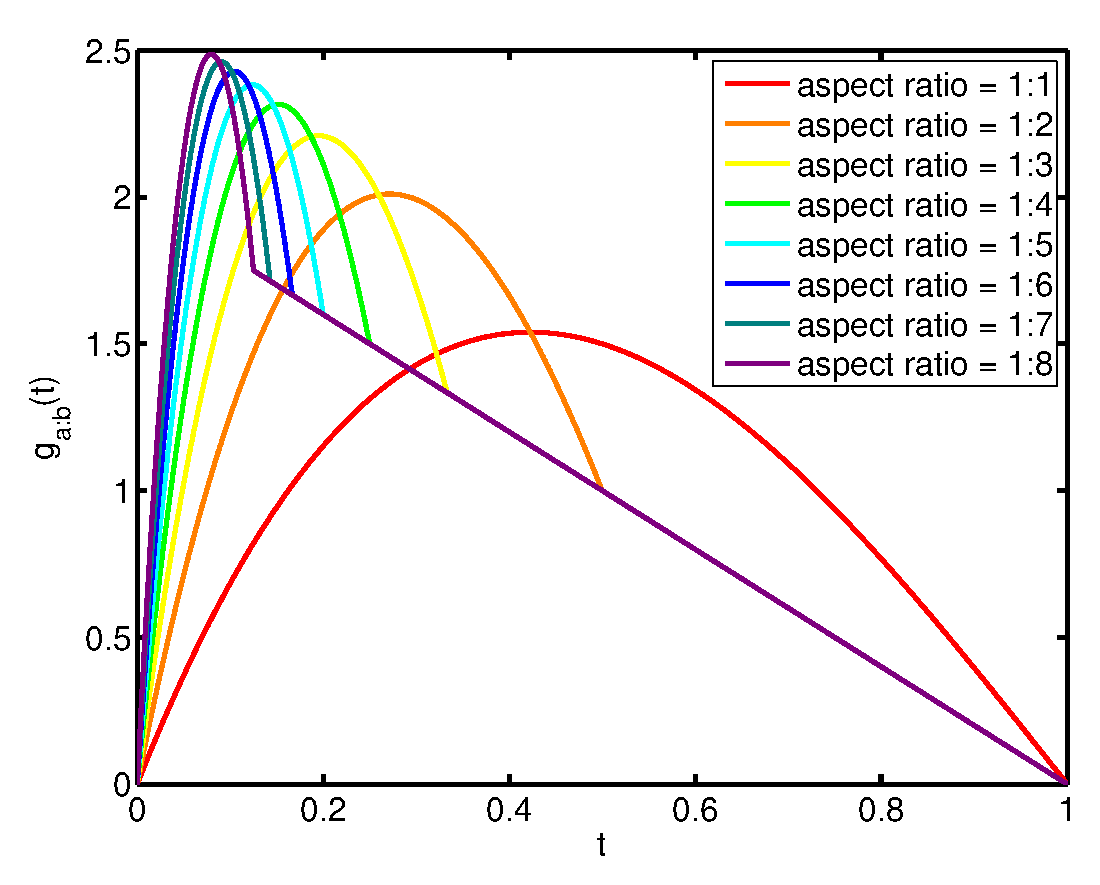
\includegraphics[width=0.48\columnwidth]{../Matlab/Plots/LinePicking_test_rect_max.eps}}
    \caption{The line picking on the rectangle with the max metric.}
  \end{center} 
\vspace{-4mm}
\end{figure}

\subsubsection{PDF}

Thus far all rectangular regions have resulted in a PDF made of three parts.
The elegant feature of this problem is that using the CDF method the rectangle 
can be partitioned into two parts. 

The  distance is the maximum of two independent random variables, i.e.,
\[ t_{\rm max} = \max (t_X,  t_Y), \]
where $t_X$ and $t_Y$ are distances given by the line-line picking
problem (Section~\ref{sec:line_line}). 

The probability density function of distances between two (uniformly) 
randomly chosen points on the unit line is given in
\eqref{eq:line_lineL}, and so the densities in the $X$ and $Y$
directions for a rectangle with sides $a$ and $b$ will be 
\begin{eqnarray}
  \label{eq:rect_xy}
  g^{\rm X}_b(t) & = & \left\{ \begin{array}{ll}
                    \frac{2}{b} \left( 1-\frac{t}{b} \right), &
                         \mbox{ for } 0 \leq t \leq b, \\
                    0, & \mbox{ otherwise}, \\
                  \end{array} \right. \nonumber \\
  g^{\rm Y}_a(t) & = & \left\{ \begin{array}{ll}
                    \frac{2}{a} \left( 1-\frac{t}{a} \right), &
                         \mbox{ for } 0 \leq t \leq a, \\
                    0, & \mbox{ otherwise}. \\
                  \end{array} \right. \nonumber 
\end{eqnarray}

Using the CDF method: 

\begin{equation}
 g^{\rm Max( X, Y)}_b(t) =
 \begin{cases}
 \frac {d  \int_{0}^{t} \int_{0}^{t}  g^{\rm X}_b g^{\rm Y}_a  dx\; dy }{dt} = \frac{2 t \left(4 a b-3 a t-3 b t+2 t^2\right)}{a^2 b^2} & 0 \le t < a \\ 
 \frac {d  \int_{0}^{a} \int_{a}^{t}  g^{\rm X}_b g^{\rm Y}_a  dx\; dy }{dt} = \frac{2 (b-t)}{b^2}& a \le t  \le b \\ 
 0 & \mbox{otherwise}
 \end{cases}
\end{equation}




\subsubsection{CDF}

The function above is comprised of two polynomial segments. A
closed form for the CDF is therefore easily derived:

\begin{equation}
 G^{\rm Max( X, Y)}_b(t) =
 \begin{cases}
 \frac{t^2 (2 a-t) (2 b-t)}{a^2 b^2} & 0 \le t < a \\ 
 \frac{t (2 b-t)}{b^2} & a \le t  \le b \\ 
 0 & t < 0\\
 1 & t > b
 \end{cases}
\end{equation}




\subsubsection{Moments}

Again because the PDF is made up of two polynomial segments calculating mean and variance is easy:

\begin{eqnarray}
 \mu &= &-\frac{a^3-5 a^2 b-10 b^3}{30 b^2}\\
 \sigma^{2} & = & -\frac{a^6-10 a^5 b+55 a^4 b^2-140 a^3 b^3+100 a^2 b^4-50 b^6}{900 b^4}
\end{eqnarray}






